\section{Result}
\markright{Result}

\begin{figure}[H]
  \centering
  \begin{subfigure}[b]{0.48\textwidth}
    \centering
    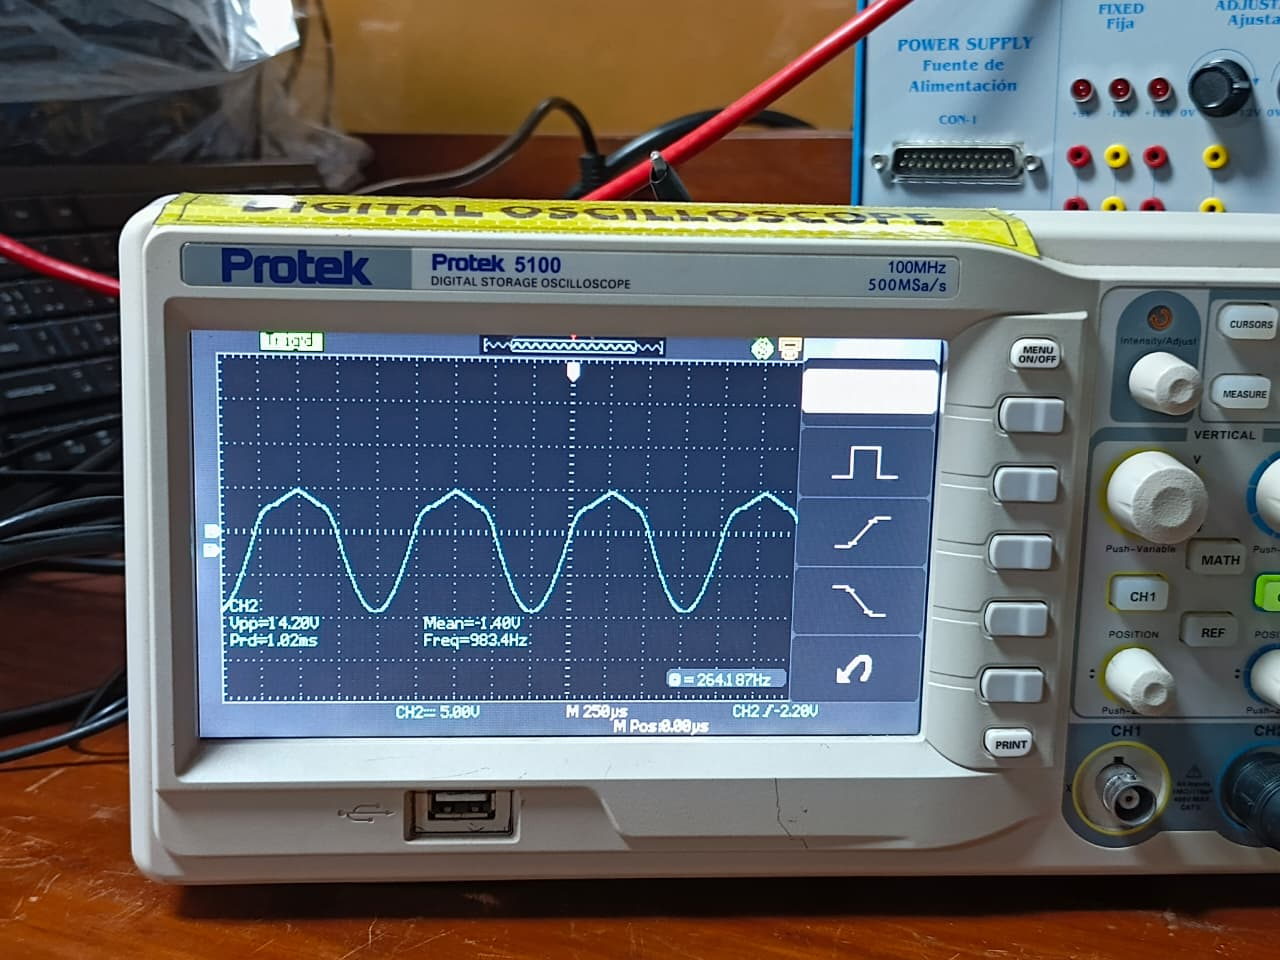
\includegraphics[width=\textwidth, height=4.5cm, keepaspectratio]{lab-03/assets/sine-input.jpeg}
    \caption{Input}
  \end{subfigure}
  \hfill
  \begin{subfigure}[b]{0.48\textwidth}
    \centering
    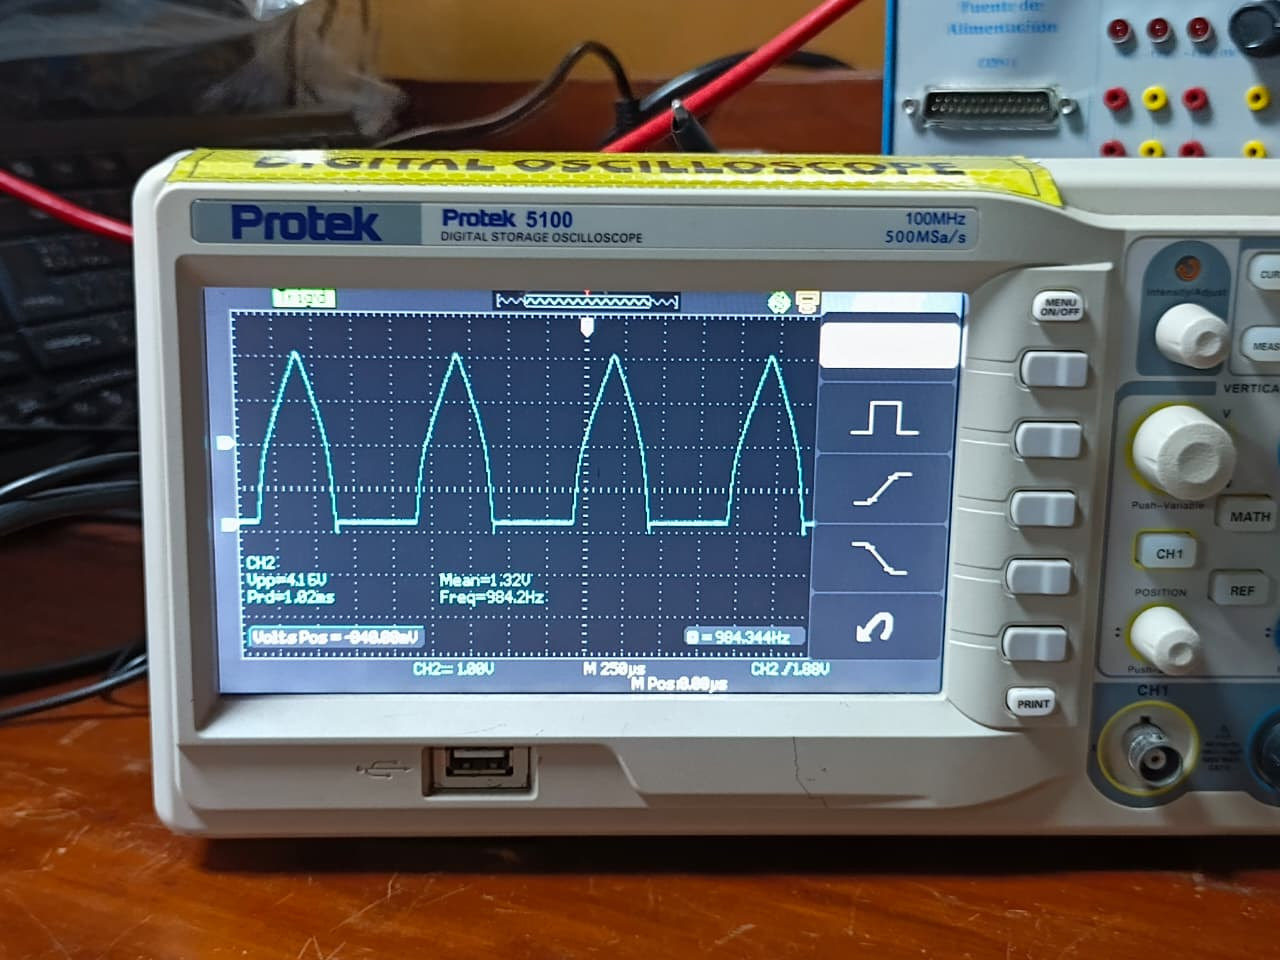
\includegraphics[width=\textwidth, height=4.5cm, keepaspectratio]{lab-03/assets/sine-output.png}
    \caption{Output}
  \end{subfigure}
  \caption{Sinusoidal wave shape in Oscillator Screen: (a) Input and (b) Output.}
  \label{fig:lab03_sine}
\end{figure}

\begin{figure}[H]
  \centering
  \begin{subfigure}[b]{0.48\textwidth}
    \centering
    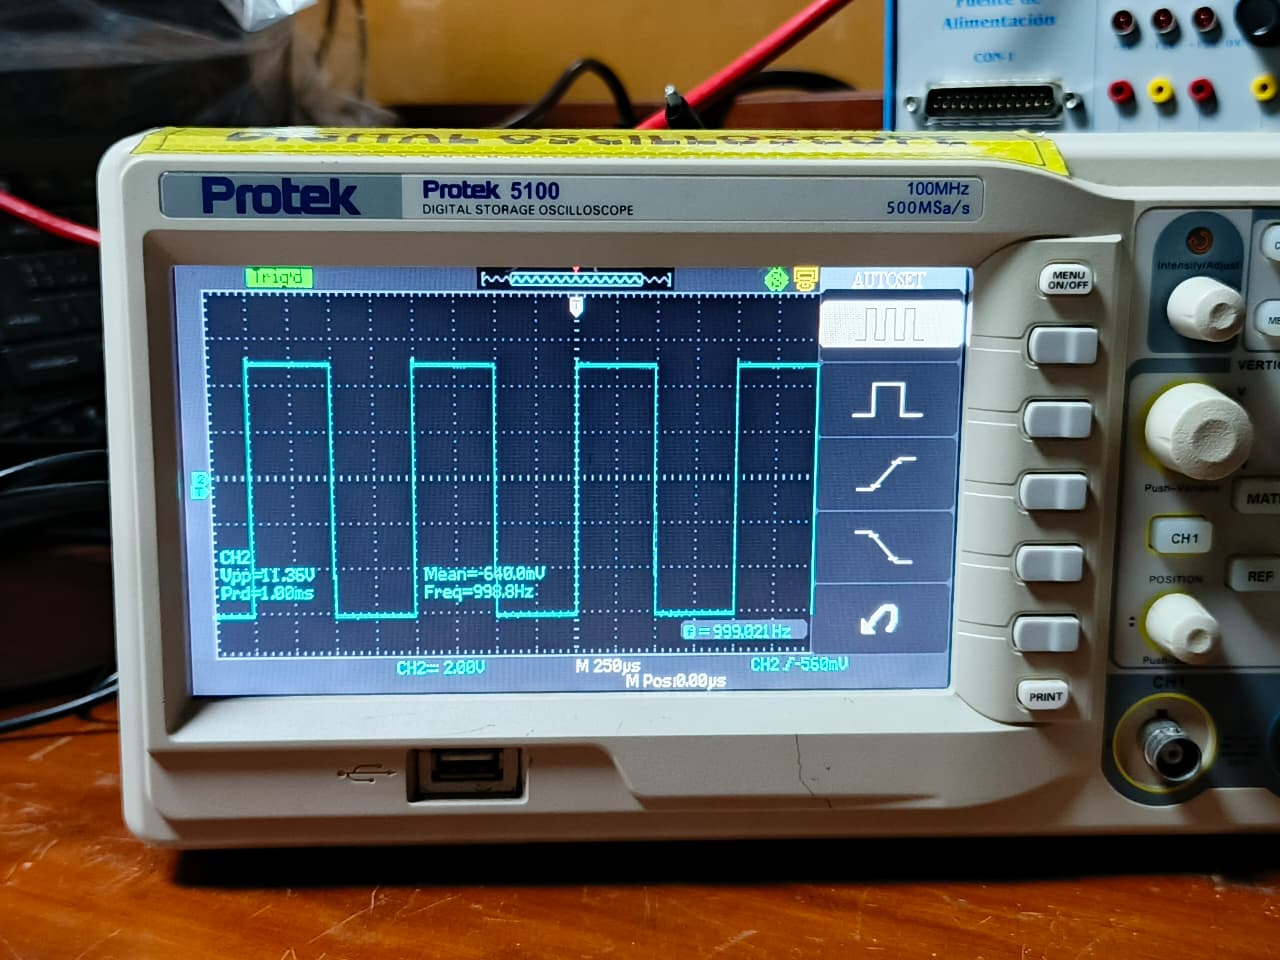
\includegraphics[width=\textwidth, height=4.5cm, keepaspectratio]{lab-03/assets/squire-input.jpeg}
    \caption{Input}
  \end{subfigure}
  \hfill
  \begin{subfigure}[b]{0.48\textwidth}
    \centering
    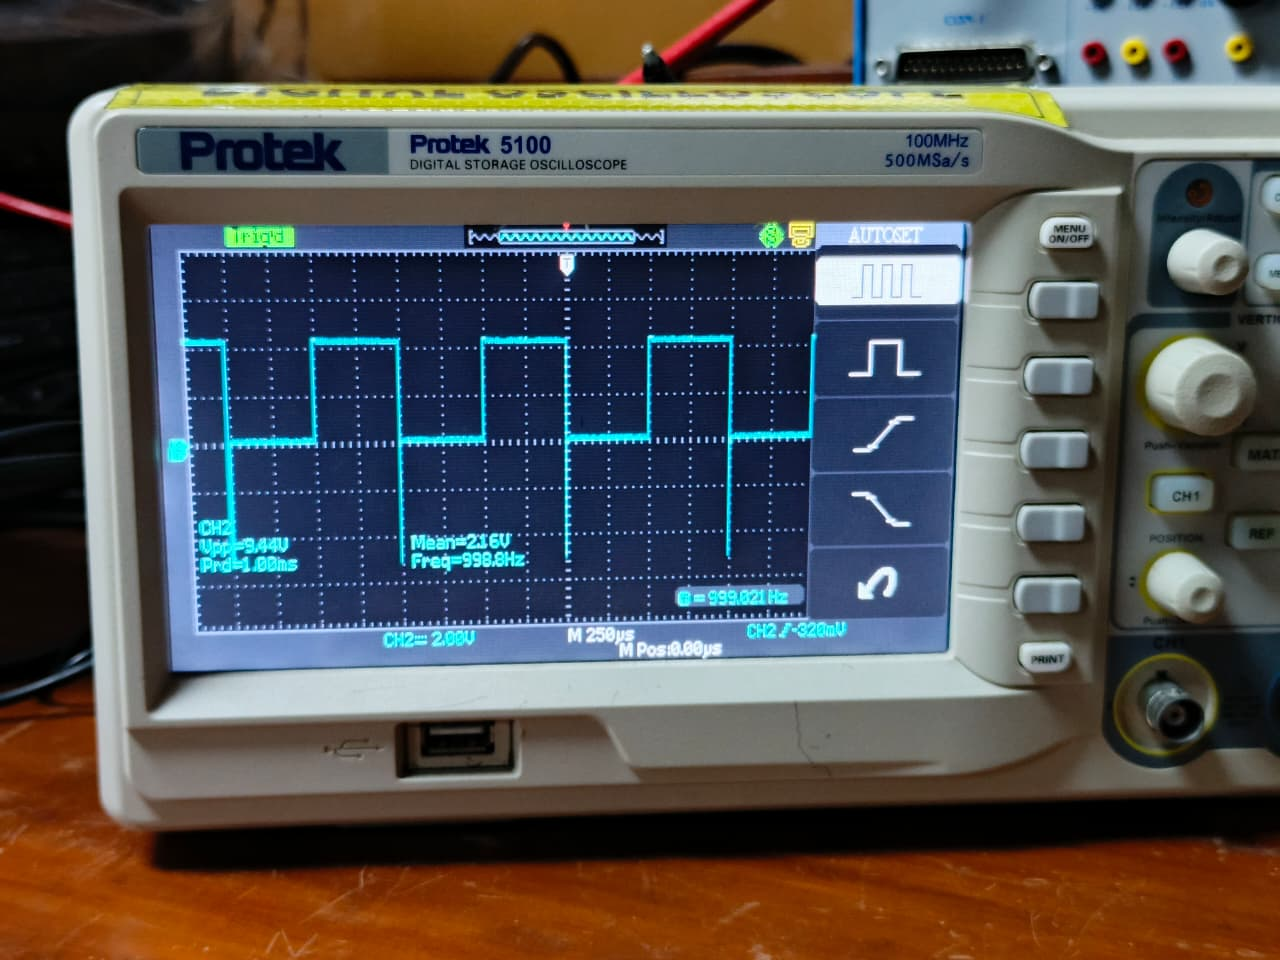
\includegraphics[width=\textwidth, height=4.5cm, keepaspectratio]{lab-03/assets/squire-output.jpeg}
    \caption{Output}
  \end{subfigure}
  \caption{Square wave shape in Oscillator Screen: (a) Input and (b) Output.}
  \label{fig:lab03_squire}
\end{figure}

\begin{figure}[H]
  \centering
  \begin{subfigure}[b]{0.48\textwidth}
    \centering
    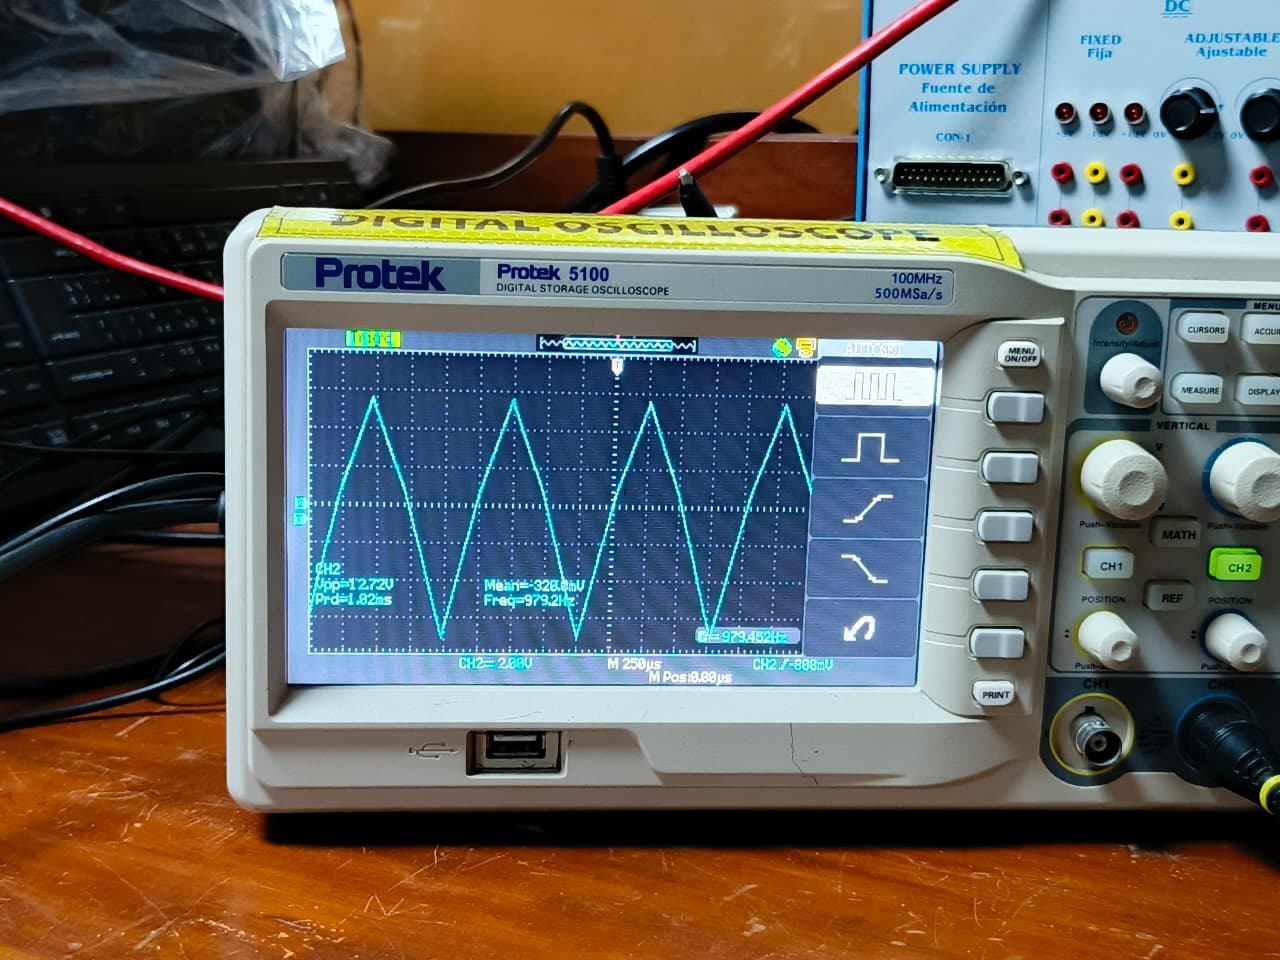
\includegraphics[width=\textwidth, height=4.5cm, keepaspectratio]{lab-03/assets/triangle-input.jpeg}
    \caption{Input}
  \end{subfigure}
  \hfill
  \begin{subfigure}[b]{0.48\textwidth}
    \centering
    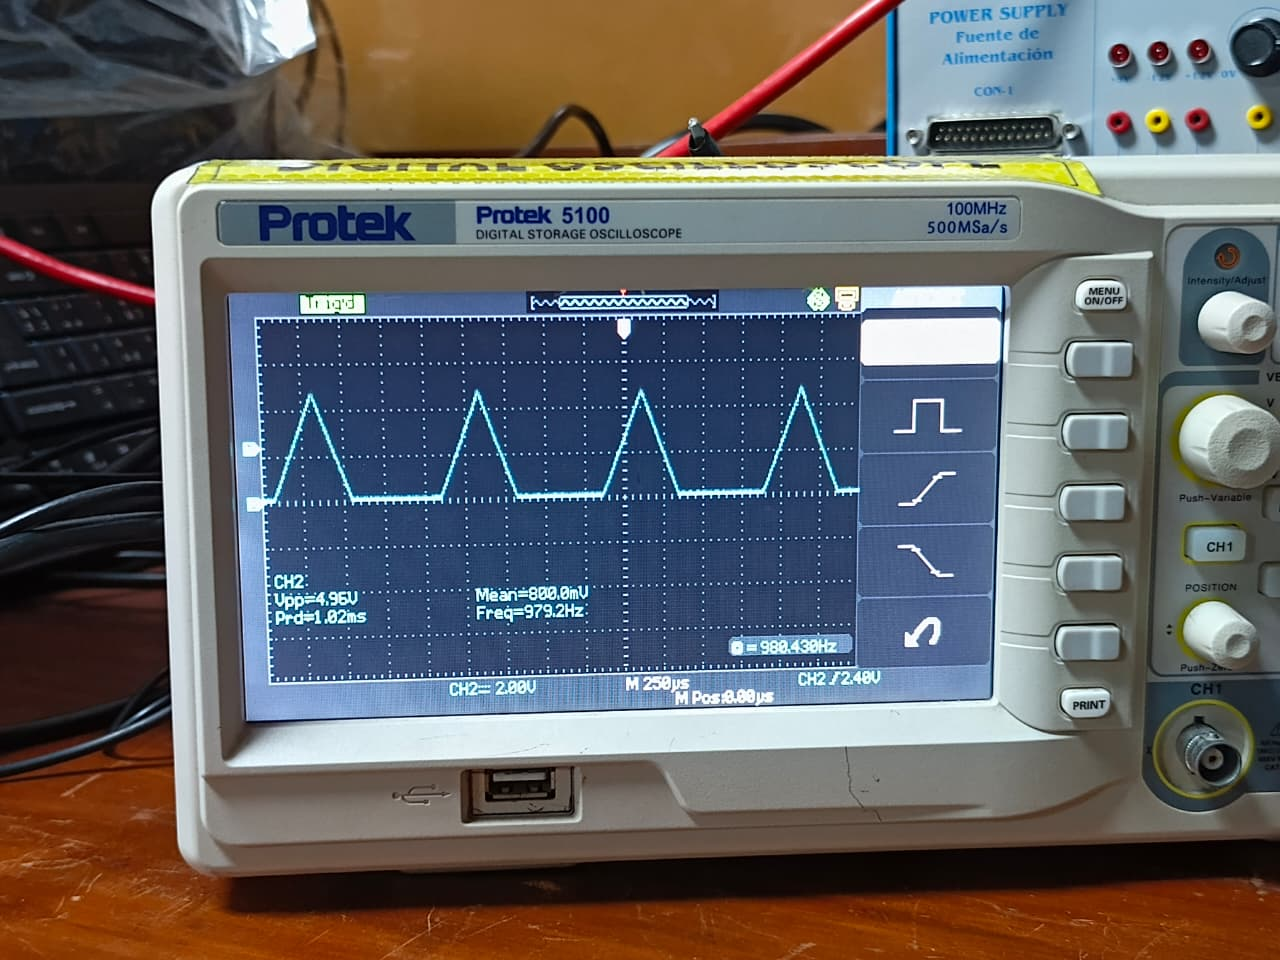
\includegraphics[width=\textwidth, height=4.5cm, keepaspectratio]{lab-03/assets/triangle-output.jpeg}
    \caption{Output}
  \end{subfigure}
  \caption{Triangular wave shape in Oscillator Screen: (a) Input and (b) Output.}
  \label{fig:lab03_triangular}
\end{figure}
